\documentclass[english]{article}



\usepackage{graphicx}
\usepackage{grffile}
\usepackage[T1]{fontenc}
\usepackage{babel}
\usepackage{float}
\usepackage{tabu}
\usepackage{ragged2e}
\usepackage{textcomp}
\usepackage{amstext}
\usepackage[final]{pdfpages}
\usepackage{caption}


\graphicspath{{Pictures/}}


\begin{document}
	
	
	\begin{figure}
		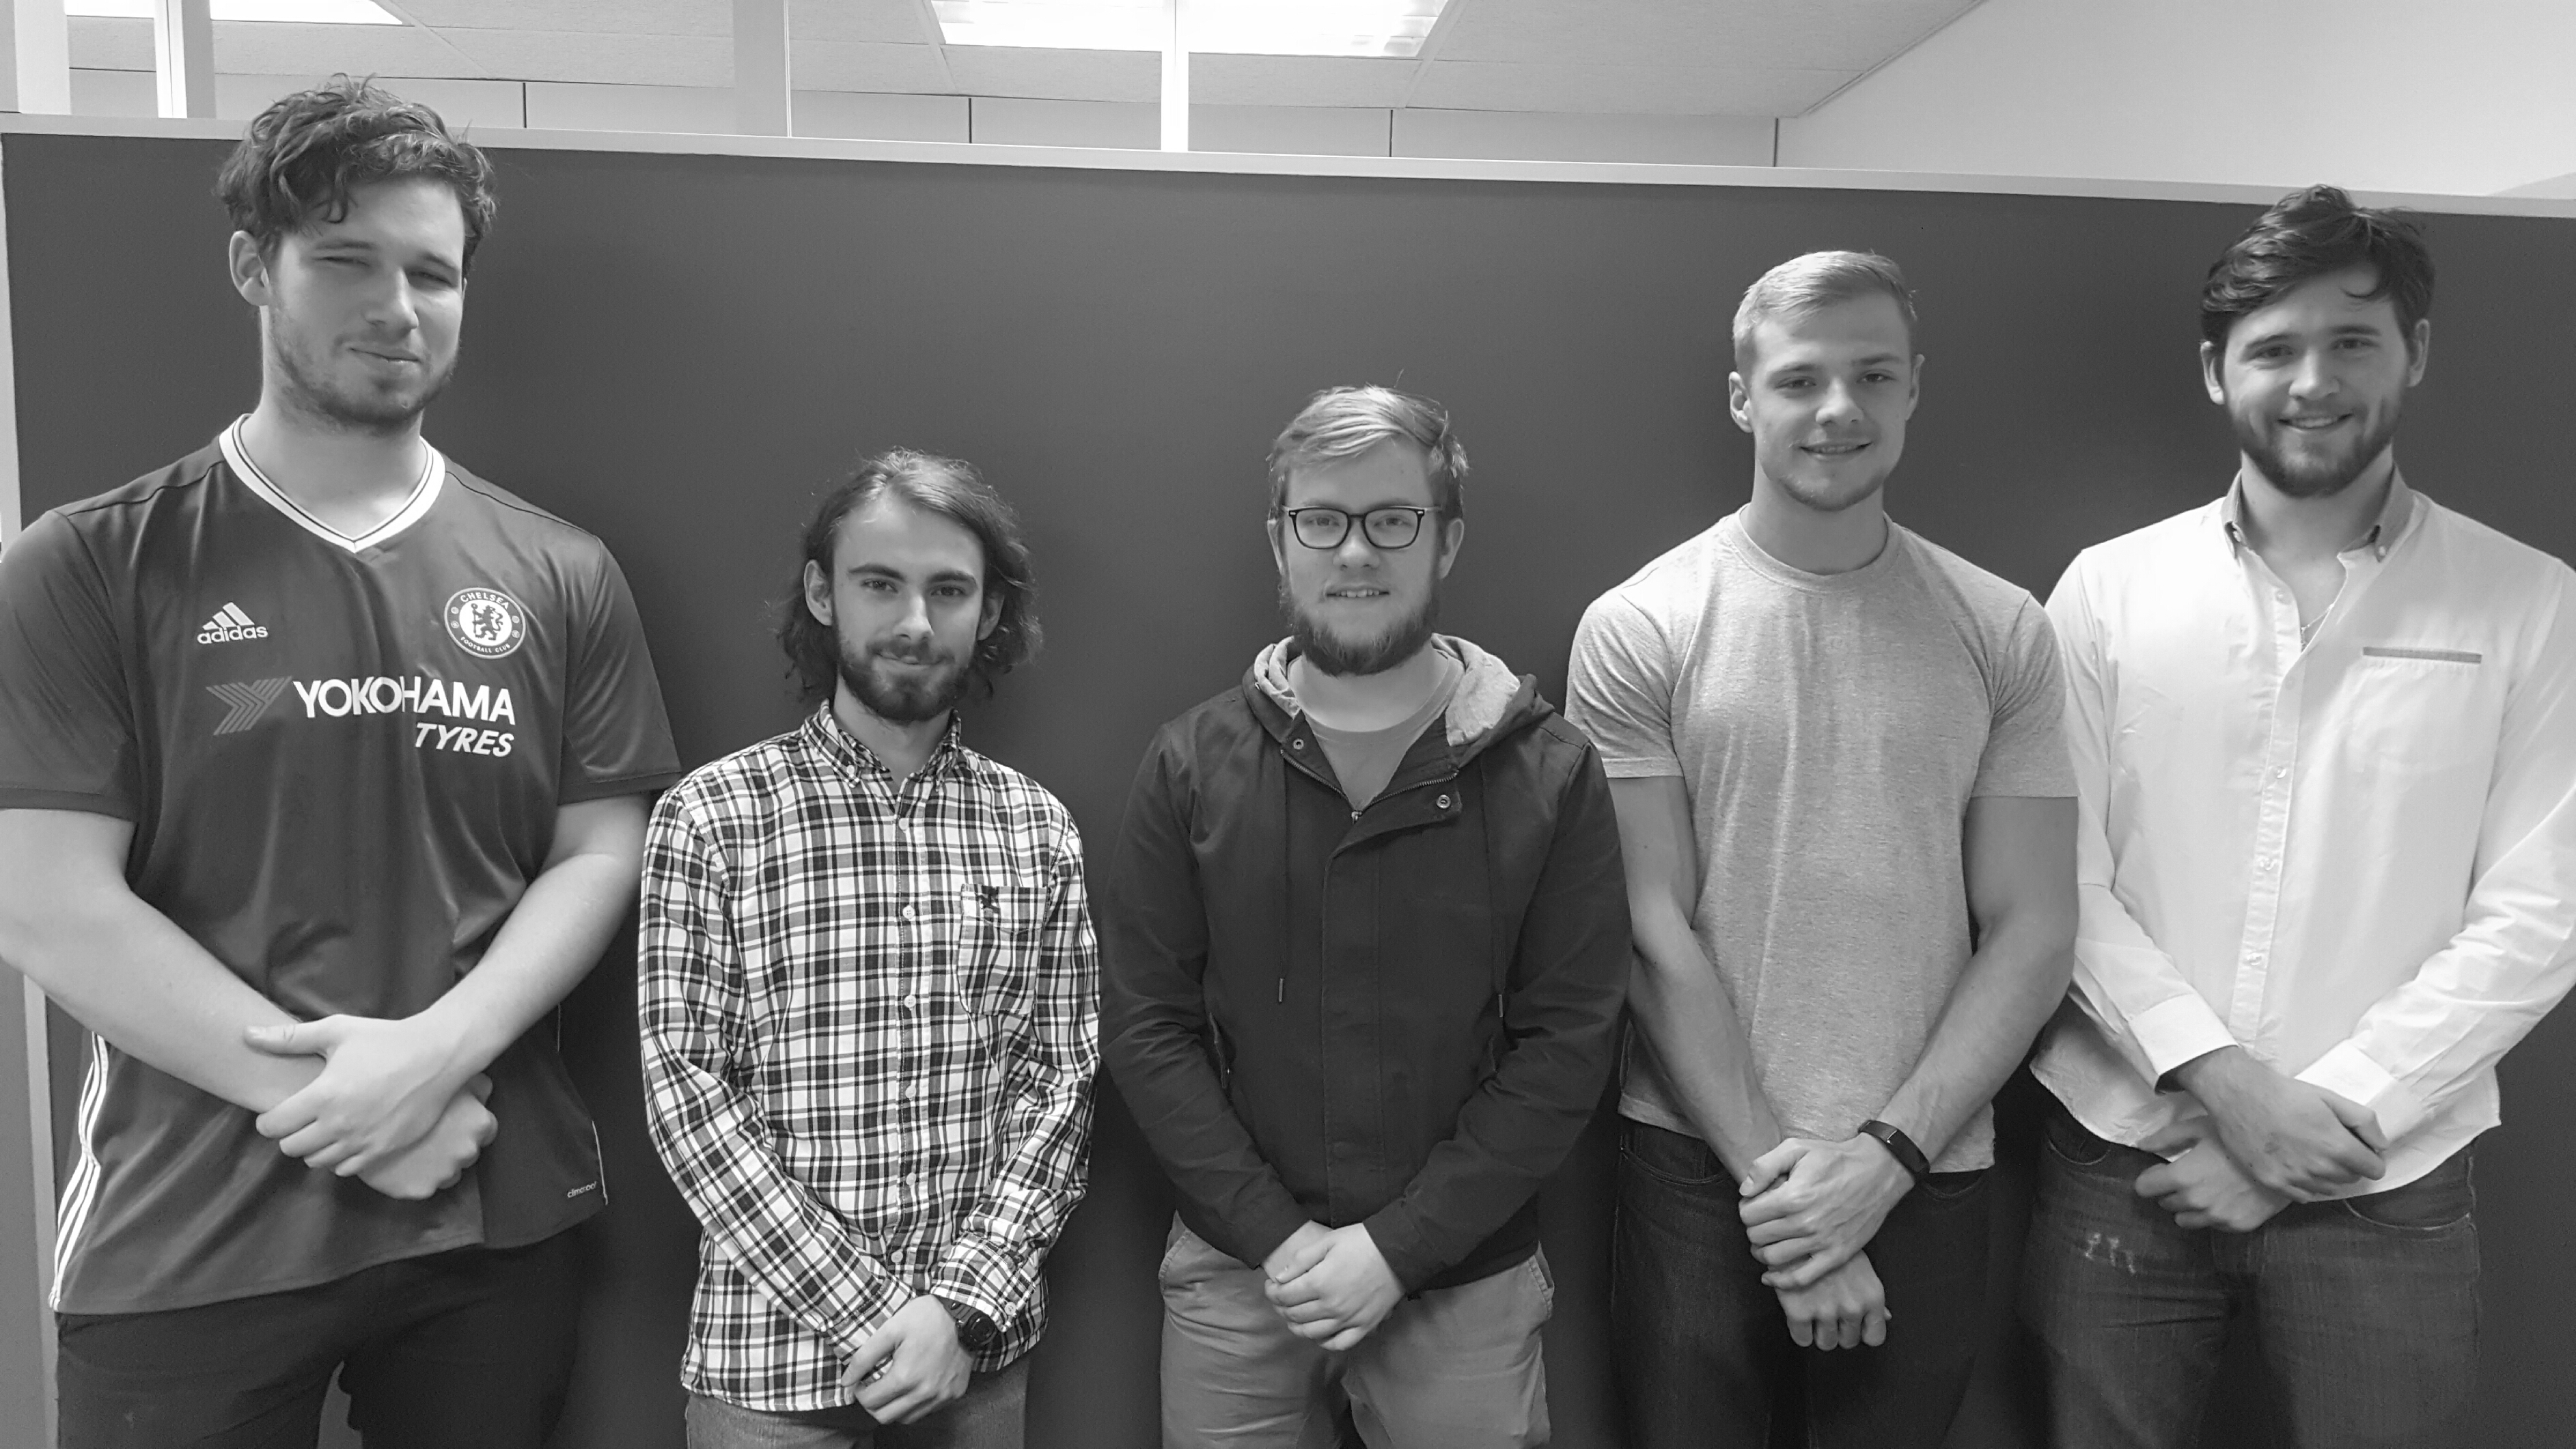
\includegraphics[width=\linewidth]{teamphoto.jpg}
	\end{figure}
	
	\begin{center}
		\line(1,0){370}
		\\[0.2cm]
		{\scshape\Large Absolute|0|  \par}
		\vspace{0.1cm}
		\line(1,0){370}
		\\[0.8cm]
		
		{\scshape\Large Voxc.js \par}
		\vspace{0.9cm}
		
		\begin{tabu} to \textwidth { X[l] X[l]}
			\hline
			\textbf{First Name, Surname  }	& \textbf{Student Number}	\\ \hline \hline
			Chris Dreyer   	&	\\ \hline
			HD HaasBroek  	&	\\ \hline
			Cameron   Trivell		&	\\ \hline
			Pearce    Jackson		&	\\ \hline
			Idrian van der Westhuizen    &15078729	\\ \hline
			\hline
		\end{tabu}
		
	\end{center}
	
	
	\pagenumbering{gobble}
	\newpage
	\tableofcontents
	
	\pagenumbering{arabic}
	\newpage

	\section*{Project details:}
	\newline
	
	\section{High level description:}
	Voxc.js is meant to be an easy to use and easy to maintain JavaScript library, from our understanding something similar to how three.js is a library for webgl. The goal of the project is to provide users a way to import voxel models into a webpage that would be using the Voxc.js library.
		\newline
	\newline
	We will use AJAX to allow users to upload the various files they plan to use such as the export from MagicaVoxel, the rules file and any additional textures they might want to add.
	\newline
\newline
	We intend to use OBJ files as both our exports from MagicaVoxel and our exports that we would be generating, as they are easier to interpret into three.js and are more commonly used. We would also be using a JSON format for our rules file, as similar to above they are easier to use directly with three.js and it’s a simpler format for users to edit in.
	\newline
\newline
	The rules file would be structured on a per colour bases and additionally on a per face or per voxel bases. The colours we will retrieve using three.js by accessing the rgb values assigned to a face and then applying the rules based on that colour. Additionally, the rules could also perhaps specify to adjust the mesh or add additional 3D models such as windows or chimneys, similar to what is seen on Oskar Stalberg’s house demo.
	\newline
\newline
	All of this will then later be deployed and demoed onto GitHub where users will be able to use the library directly, but effectively the goal is to allow it to be used on any other website as a plug-in library.
	\medskip
	
	\section{Deployment diagram:}
	\medskip
	\section{Brief description of methodology:}
	
	We will be developing according to a feature driven development agile methodology, as there are various features within the scope of the Voxc.js library to be implemented, and some can be developed separately from the rest, while others might depend on the outcome of a previous feature, for instance one feature is the ability to import a file into the library that was created using MagicaVoxel, but another feature is where we export the mesh we created, both separate features, but the first has to work correctly before we can move onto the second.
		\newline
	\newline
	This methodology also allows us as a team to focus on current tasks and the most important features first. It also allows us to get better feedback from the client more frequently as they only have to test the most newly developed feature.
		\newline
	\newline
	For this reason, we will be having team meetings twice a week, once on Monday and the second on Thursday. The meetings will be used to discuss which feature to develop next and how to split into sub-teams if needed, additionally every other meeting will be used as a progress report and testing phase for the current features, and all previous features to make sure the newly added features do not conflict with any other ones. We would also like to hold meetings with the client once a feature has finished development on our end to see if it works as expected and if it was what the client wanted. This process will run iteratively as they will be repeated until the client is satisfied with the delivered feature.  
	\medskip
	\section{Team skills:}
	Two of our members have graphics as a subject, thus we already know how webgl and three.js works so we don't have to learn from scratch.
	\newline
	\newline
	Additionally the other 3 members are skilled at more logical programming as well as the use of AJAX and web development in general. This will allows us to create a user friendly and dynamic interface for the library.
	\newline
	\newline
	One of our members also knows photoshop and blender, thus we can make our own textures and/or models to be added to the Voxc.js library without having to worry about copyright.
	\medskip
	
\end{document}          
